\documentclass{article}

\usepackage{booktabs}
\usepackage{tabularx}
\usepackage{graphicx}

\title{SE 3XA3: Development Plan\\OpenCameraRefined}

\author{Team 211, Team Elon
		\\ Pedram Yazdinia, yazdinip
		\\ Zayed Sheet, sheetz
		\\ Faisal Jaffer, jaffem1
		\\ Dominik Buszowiecki, buszowid 
}

\date{\today}

%\input{../Comments}

\begin{document}

\begin{table}[hp]
\caption{Revision History} \label{TblRevisionHistory}
\begin{tabularx}{\textwidth}{llX}
\toprule
\textbf{Date} & \textbf{Developer(s)} & \textbf{Change}\\
\midrule
Date1 & Name(s) & Description of changes\\
Date2 & Name(s) & Description of changes\\
... & ... & ...\\
\bottomrule
\end{tabularx}
\end{table}

\newpage

\maketitle


This document contains the development plan for the implementation of ''OpenCamera”. The intent of this document is to set appropriate meeting times and a working communication plan that is feasible to all members of the group. It also set the styles standards by which the code shall be written and pushed to git. Each member is assigned a role and tasks that they must complete and update the progress to the team in the weekly set meetings.


\section{Team Meeting Plan}

In addition to the lab times where all members do tutorial work and improve the project, each group member is responsible for consistent presence in weekly online and personal meetings. These meetings take place every Monday and Saturday with different purposes. Saturday meetings take place to bring every person of the group uptodate while evaluating the progress done over the week. These meetings are brief and take place over online platforms(Facebook Messenger). Monday meetings provide a chance for the developers to discuss, design and implement on any aspect of the product. It is very crucial that developers personally attend these meetings. These meetings usually take around an hour, within study rooms of Thode Library. Within the group, Zayed Sheet will take control over the structure of each agenda as the group chair. He will ensure that the meeting flows as planned through agenda and that each member is informed of their “homework”. Finally, he is responsible for gathering the written statement of the decisions made. 

\section{Team Communication Plan}

In order to ensure all members are up to date with the project, the team will be communicating through a Facebook Messenger group. Whenever a team member decides to work on a portion of the project, they will be required to inform the group about what they are about to do. This is to ensure that there are no conflicts or overlap between the work done among group members. The messenger group will also be used to plan meetings or inform the others if they cannot make the meetings.

\section{Team Member Roles}

\begin{table}[h]
\begin{tabular}{|l|l|}
\hline
\textbf{Group Member} & \textbf{Role}                   \\ \hline
Pedram Yazdinia       & Git expert, LaTex expert        \\ \hline
Dominik Buszowiecki   & Java Expert, Latex expert       \\ \hline
Faisal Jaffer         & Group Leader, Java Expert       \\ \hline
Zayed Sheet           & Tensorflow expert, Latex expert \\ \hline
\end{tabular}
\end{table}
\section{Git Workflow Plan}

The original open source project will be cloned as OpenCameraRefined in GitLab. Since our team has a single important feature, will use the Feature Branch workflow to maintain our codebase on Git. Each member will work on the same branch, solving different issues that need to be addressed. Each commit is going to be assigned a solution label that targets the problem that it has addressed. When the feature has been implemented on the branch, it will be merged into the master branch.
\section{Proof of Concept Demonstration Plan}

The proof of concept will surely be one of the most stressful parts of the assignment, however with proper planning and preparation we can minimize any risks or unexpected events. 

The addition of a picture auto capture feature will be risky because of the machine learning models that will need to be implemented for it to work. The plan to demonstrate the feasibility of this feature is to show a working concept of a machine learning model that can successfully distinguish between different gestures. This does not have to be directly incorporated in the app at this stage.

Because our app runs on a separate environment it will require android studio. Integration between the Java code and the android platform will need to be experimented a week in advance to ensure familiarity within the environment. We will use Zayed Sheet’s android mobile device to experiment with the environment and demonstrate the proof of concept. 

Lastly, testing will be a vital component to ensure the smoothness of the demonstration. We will use unit testing software such as JUnit version 5 for a more efficient process. In addition, we will use the android studio Emulator to test features wherever possible, in order to reduce the time for switching between environments. 


\section{Technology}

The application will be written using Java with the Android Studio IDE. Android Studio will be used as it features a built in device emulator to allow testing to be performed on various devices and android versions. On top of this, we plan to test the application a real device which is another feature that Android Studio offers. In order to produce documentation, the IDE includes a built in JavaDoc generator which will read the JavaDoc comments that our team will have written in the code.

\section{Coding Style}

Consistency between coding styles throughout the project is important in order for all group members to be able to revise and review other group member’s code. This is why all our project code will follow the “Google Java Style Guide”

\section{Project Schedule}

\begin{figure}[h!]
\centering
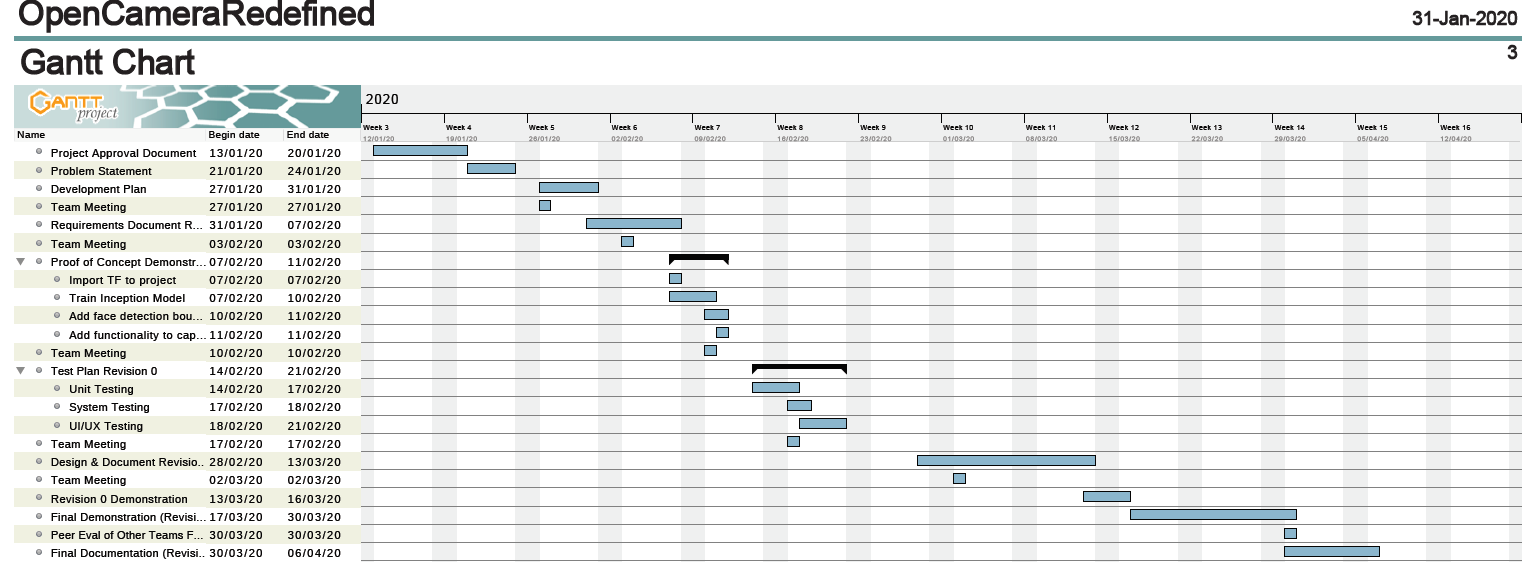
\includegraphics[width=50mm, scale = 2]{Gantt}
\caption{Gantt}
\label{fig:method}
\end{figure}
The Doc folder contains a more detailed Gantt.pdf which includes more information. 

\section{Project Review}

\end{document}